\documentclass[11pt,a4paper]{article}

% ─── Codificação e idioma ────────────────────────────────────────────────────
\usepackage[utf8]{inputenc}
\usepackage[T1]{fontenc}
\usepackage[portuguese]{babel}
\usepackage{lmodern}

% ─── Layout ──────────────────────────────────────────────────────────────────
\usepackage[a4paper,margin=2.5cm]{geometry}
\usepackage{microtype}
\usepackage{setspace}
\onehalfspacing
\usepackage{parskip}

% ─── Figuras e tabelas ───────────────────────────────────────────────────────
\usepackage{graphicx}
\usepackage{float}
\usepackage{booktabs}
\usepackage{array}
\usepackage{multirow}
\usepackage{caption}
\captionsetup{font=small,labelfont=bf}
\graphicspath{{figuras/}}

% ─── Código e pseudo-código ──────────────────────────────────────────────────
\usepackage{listings}
\usepackage{xcolor}
\usepackage[ruled,vlined,linesnumbered]{algorithm2e}
\definecolor{codebg}{rgb}{0.97,0.97,0.97}
\definecolor{codekw}{rgb}{0.10,0.10,0.60}
\definecolor{codecm}{rgb}{0.30,0.55,0.30}
\lstset{
  basicstyle=\ttfamily\footnotesize,
  backgroundcolor=\color{codebg},
  keywordstyle=\color{codekw}\bfseries,
  commentstyle=\color{codecm}\itshape,
  breaklines=true,
  frame=single,
  showstringspaces=false,
  numbers=left,
  numberstyle=\tiny,
  language=Python,
}

% ─── Matemática e hyperlinks ─────────────────────────────────────────────────
\usepackage{amsmath,amssymb}
\usepackage[hidelinks]{hyperref}
\usepackage{enumitem}

% ─── Macro para marcar texto ainda por escrever ──────────────────────────────
\newcommand{\todo}[1]{\par\noindent\textcolor{red}{\small[\textbf{TODO:} #1]}\par}

% ═════════════════════════════════════════════════════════════════════════════
\begin{document}

% ─── Capa ────────────────────────────────────────────────────────────────────
\begin{titlepage}
  \centering
  \vspace*{1.5cm}
  {\Large\textsc{Universidade de Aveiro}}\\[0.3cm]
  {\large Departamento de Eletrónica, Telecomunicações e Informática}\\[2.5cm]

  {\large Redes e Sistemas Autónomos}\\[1.5cm]

  \rule{\linewidth}{0.4mm}\\[0.6cm]
  {\Huge\bfseries Cooperative Lane Merge\\[0.3cm]}
  {\Large via Comunicação V2V}\\[0.4cm]
  \rule{\linewidth}{0.4mm}\\[1.5cm]

  {\large\itshape Sistema autónomo de apoio à inserção cooperativa em faixa de rodagem}\\[3cm]

  {\large Pedro Melo \quad n.º 114208}\\[2cm]

  {\large \today}\\[1cm]

  \begin{tabular}{rl}
    \textbf{Repositório:} & \href{https://example.com}{\color{blue}(inserir URL)} \\[0.2cm]
    \textbf{Vídeo da demo:} & \href{https://example.com}{\color{blue}(inserir URL / Discord)} \\
  \end{tabular}
\end{titlepage}

\tableofcontents
\newpage

% ═════════════════════════════════════════════════════════════════════════════
\section{Introdução}
\label{sec:intro}

O aumento da densidade de tráfego nas entradas de autoestrada torna a inserção de
veículos provenientes de rampas de acesso um dos pontos mais críticos para a fluidez
e a segurança rodoviária. Tradicionalmente, esta manobra depende do julgamento
individual de cada condutor, o que frequentemente origina travagens bruscas, paragens
na rampa ou inserções forçadas que propagam ondas de congestionamento para a via
principal.

Este projeto, desenvolvido no âmbito da unidade curricular de Redes e Sistemas
Autónomos, explora como a comunicação Veículo-a-Veículo (V2V) pode substituir esse
julgamento individual por uma \textbf{negociação cooperativa e distribuída}, sem
qualquer entidade central de controlo. O cenário estudado é o de um veículo --- o
\emph{Merge Car} (MC) --- que se aproxima da via principal a partir de uma rampa de
acesso e necessita de coordenar a sua inserção com os veículos que já circulam nessa
via. Em vez de impor a sua entrada, o MC inicia um protocolo de coordenação de manobra
em que os veículos afetados são identificados em tempo real, decidem cooperativamente
um abrandamento controlado e concedem ao MC uma janela temporal segura para a inserção.

A solução assenta integralmente em mensagens normalizadas ETSI C-ITS:
\emph{Cooperative Awareness Messages} (CAM) para a consciência situacional periódica e
\emph{Manoeuvre Coordination Messages} (MCM) para a negociação da manobra. A pilha de
comunicação é fornecida pelo Vanetza-NAP, o transporte de mensagens pelo middleware
Zenoh, e toda a lógica dos veículos corre em containers Docker independentes,
garantindo que cada veículo é um nó autónomo que só conhece a sua vizinhança através
das CAMs que recebe. Uma dashboard web em tempo real permite observar a negociação e a
manobra à medida que decorrem.

Este relatório descreve os objetivos do trabalho (Secção~\ref{sec:objetivos}), a
arquitetura do sistema (Secção~\ref{sec:arquitetura}), a implementação detalhada do
protocolo e dos algoritmos de decisão (Secção~\ref{sec:implementacao}), o fluxo da
demonstração (Secção~\ref{sec:demo}) e os resultados obtidos nos vários cenários
testados (Secção~\ref{sec:resultados}), incluindo casos com dois veículos a inserir-se
em simultâneo.

% ═════════════════════════════════════════════════════════════════════════════
\section{Objetivos}
\label{sec:objetivos}

\subsection{Problema}

A inserção de um veículo proveniente de uma rampa de acesso na via principal é uma das
manobras com maior potencial de conflito da circulação rodoviária. Sem cooperação entre
veículos, o condutor que vem da rampa só dispõe da sua própria perceção visual para
encontrar uma folga: quando esta não existe, vê-se obrigado a forçar a entrada, a travar
bruscamente ou mesmo a parar no final da rampa à espera de espaço. Cada uma destas
reações tem custos:

\begin{itemize}[noitemsep,topsep=2pt]
  \item \textbf{Inserção forçada} --- obriga os veículos da via principal a travagens de
        emergência, comprometendo a segurança;
  \item \textbf{Paragem na rampa} --- elimina a velocidade de aproximação necessária para
        uma inserção suave e cria risco de colisão traseira na própria rampa;
  \item \textbf{Travagens reativas} --- propagam-se para montante sob a forma de ondas de
        choque, degradando a fluidez de todo o troço.
\end{itemize}

A raiz do problema é a \emph{falta de informação antecipada e de coordenação}: os
veículos da via principal só percebem a intenção de inserção quando o veículo da rampa já
está praticamente sobre o ponto de conflito, deixando pouca margem para uma resposta
suave.

\subsection{Objetivo geral}

O objetivo central deste trabalho é demonstrar que a comunicação Veículo-a-Veículo (V2V)
permite resolver este problema através de uma \textbf{negociação cooperativa, distribuída
e antecipada}, sem qualquer entidade central de controlo e assente exclusivamente em
mensagens normalizadas ETSI C-ITS (CAM e MCM). Pretende-se que o veículo da rampa --- o
\emph{Merge Car} (MC) --- anuncie a sua intenção com antecedência suficiente para que os
veículos afetados se ajustem de forma coordenada e lhe abram uma janela temporal segura,
substituindo a reação tardia por uma manobra planeada.

\subsection{Objetivos específicos}

Para concretizar o objetivo geral, definiram-se os seguintes objetivos específicos:

\begin{enumerate}[noitemsep,topsep=2pt,label=\textbf{O\arabic*.}]
  \item \textbf{Consciência situacional contínua} --- cada veículo difunde periodicamente
        a sua posição, velocidade, aceleração e dimensões via CAM, construindo uma visão
        local do tráfego sem qualquer configuração prévia da vizinhança.
  \item \textbf{Protocolo de negociação de manobra} --- definir e implementar um protocolo
        distribuído sobre MCM que permita ao MC pedir autorização e aos restantes veículos
        responder cooperativamente.
  \item \textbf{Deteção de conflito} --- determinar, em cada veículo da via principal e em
        tempo real, se irá efetivamente partilhar a zona de conflito com o MC, combinando
        a geometria da estrada com uma janela temporal de ocupação.
  \item \textbf{Abrandamento coordenado em cadeia} --- quando há conflito, calcular uma
        velocidade-alvo viável e propagar o pedido de abrandamento aos veículos a montante,
        de modo a abrir a folga necessária sem travagens bruscas.
  \item \textbf{Garantia de segurança} --- assegurar que a manobra nunca compromete a
        segurança: se a negociação não concluir a tempo, o MC recorre a um mecanismo de
        \emph{stop-and-wait} no final da rampa e volta a tentar.
  \item \textbf{Suporte a múltiplos veículos a inserir-se} --- estender o protocolo a
        cenários com dois veículos a fundir-se simultaneamente a partir da rampa.
  \item \textbf{Observabilidade} --- disponibilizar uma visualização em tempo real da
        simulação e da troca de mensagens, para validação e demonstração do protocolo.
\end{enumerate}

\subsection{Síntese}

A Tabela~\ref{tab:objetivos} resume como cada objetivo específico é concretizado na
implementação, remetendo para a secção correspondente.

\begin{table}[H]
  \centering
  \small
  \renewcommand{\arraystretch}{1.25}
  \begin{tabular}{@{}p{0.34\linewidth}p{0.50\linewidth}c@{}}
    \toprule
    \textbf{Objetivo} & \textbf{Mecanismo de concretização} & \textbf{Secção} \\
    \midrule
    O1 -- Consciência situacional &
      Beaconing CAM a 100\,ms + \texttt{NeighbourTable} com janela de 200\,ms &
      \ref{sec:implementacao} \\
    O2 -- Protocolo de negociação &
      6 subtipos de MCM (\textsc{merge\_request}, \textsc{slowdown\_request/grant},
      \textsc{merge\_grant}, \textsc{merge\_confirmed}, \textsc{execution\_status}) &
      \ref{sec:implementacao} \\
    O3 -- Deteção de conflito &
      Projeção geométrica (\texttt{project\_t}) + sobreposição temporal entre a ocupação
      do MC e a entrada/saída do veículo na zona &
      \ref{sec:implementacao} \\
    O4 -- Abrandamento em cadeia &
      Velocidade-alvo por busca binária (\texttt{\_solve\_target\_speed}) e propagação de
      \textsc{slowdown\_request} ao veículo de trás &
      \ref{sec:implementacao} \\
    O5 -- Garantia de segurança &
      Verificação cinemática de travagem (\texttt{can\_brake\_in\_time}) e paragem em
      \texttt{stop\_t} com retentativa &
      \ref{sec:implementacao} \\
    O6 -- Múltiplos MC &
      Mesmo protocolo na rampa: o MC propaga \textsc{slowdown\_request} ao veículo atrás
      na rampa &
      \ref{sec:implementacao} \\
    O7 -- Observabilidade &
      Ponte Zenoh$\rightarrow$WebSocket (\texttt{bridge.py}) e dashboard HTML em tempo real &
      \ref{sec:implementacao} \\
    \bottomrule
  \end{tabular}
  \caption{Mapeamento dos objetivos específicos para os mecanismos de implementação.}
  \label{tab:objetivos}
\end{table}

% ═════════════════════════════════════════════════════════════════════════════
\section{Arquitetura}
\label{sec:arquitetura}

O sistema está organizado em quatro camadas com responsabilidades bem separadas, tal
como ilustra a Figura~\ref{fig:arch}. Esta secção fixa o vocabulário (nós, papéis,
tópicos e mensagens) que a Secção~\ref{sec:implementacao} utiliza para detalhar a
implementação.

\subsection{Visão geral em camadas}

\begin{figure}[H]
  \centering
  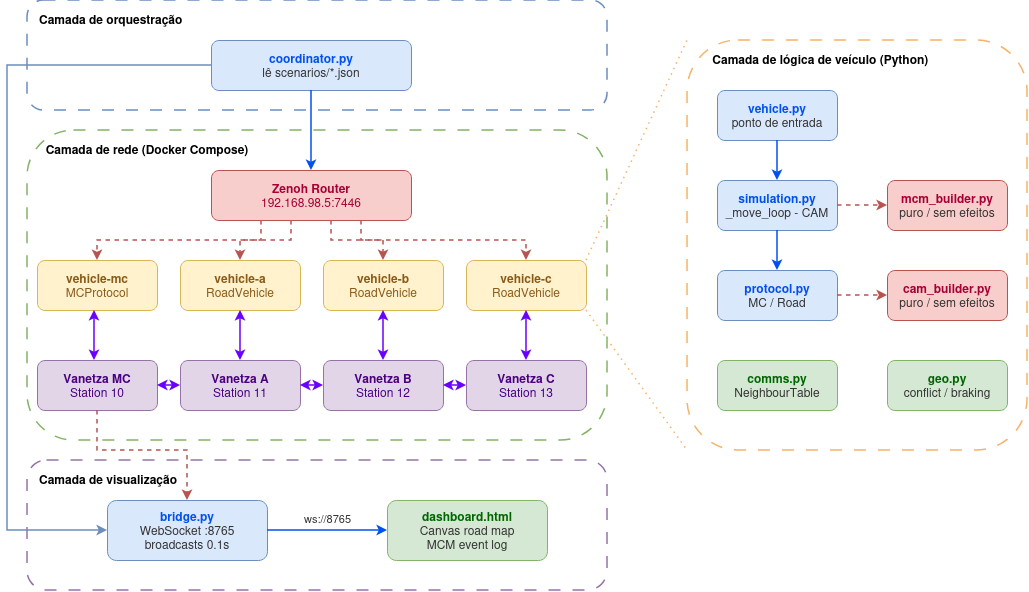
\includegraphics[width=\linewidth]{MERGE_LANE_ARCH.png}
  \caption{Arquitetura em camadas do sistema.}
  \label{fig:arch}
\end{figure}

\begin{description}[leftmargin=1.4em,topsep=2pt,itemsep=3pt]
  \item[\textbf{Camada de orquestração.}] Um único processo, o \texttt{coordinator.py}
        (GUI Tkinter), lê os ficheiros de cenário \texttt{scenarios/*.json}, publica o
        cenário escolhido no router Zenoh e aguarda que todos os veículos ativos
        reportem a conclusão. É o ponto de entrada da demonstração, mas \emph{não}
        participa na negociação --- apenas dá o pontapé de saída e recolhe o estado de
        cada veículo.
  \item[\textbf{Camada de rede.}] Materializada por \texttt{docker-compose} sobre a
        rede Docker externa \texttt{vanetzalan0}. Contém o \emph{router Zenoh}
        (canal do coordinator) e, por cada veículo, um par de containers: um container
        \textbf{Vanetza-NAP}, que implementa a pilha ETSI C-ITS (codificação/
        descodificação ASN.1 e difusão pelo ``ar''), e um container \textbf{Python},
        que corre a lógica do veículo. É nesta camada que vivem as \emph{stations}
        10--13.
  \item[\textbf{Camada de lógica de veículo (Python).}] É o cérebro de cada nó,
        organizado em módulos: \texttt{vehicle.py} (ponto de entrada),
        \texttt{simulation.py} (laço de movimento e emissão de CAM),
        \texttt{protocol.py} (a classe \texttt{MergeProtocol}, que concentra toda a
        negociação), apoiados por \texttt{geo.py} (geometria e modelo de travagem),
        \texttt{comms.py} (sessões Zenoh e \texttt{NeighbourTable}) e pelos
        construtores puros de mensagens \texttt{cam\_builder.py} e
        \texttt{mcm\_builder.py}. Esta camada é o objeto central da
        Secção~\ref{sec:implementacao}.
  \item[\textbf{Camada de visualização.}] O \texttt{bridge.py} subscreve o tráfego V2X
        (CAM e MCM) descodificado, mantém o estado de cada veículo e difunde, a cada
        100\,ms, uma trama JSON por WebSocket (porta 8765) para a
        \texttt{dashboard.html}, que desenha as estradas, os veículos e o registo de
        eventos MCM em tempo real.
\end{description}

\paragraph{Os dois planos de comunicação.} A Figura~\ref{fig:arch} distingue, por cor,
dois planos. O \emph{plano V2X} (ligações entre cada veículo e o seu Vanetza e entre os
Vanetza) transporta o tráfego C-ITS (CAM/MCM) e representa o meio rádio: na realidade,
cada veículo difunde-o pelo broker Zenoh do seu \emph{próprio} container Vanetza-NAP
(\texttt{tcp/<ip>:7447}) --- não existe broker partilhado para o V2X, e a figura abstrai
esses brokers como ligações diretas. O \emph{plano de orquestração} (ligações ao bloco
central ``Zenoh Router'', \texttt{192.168.98.5:7446}) transporta apenas as mensagens de
controlo da demonstração (cenário, \emph{ready}, \emph{done}). Assim, nenhum veículo
comunica com outro por um canal partilhado privilegiado --- toda a coordenação
inter-veicular acontece exclusivamente através de mensagens C-ITS difundidas pelo
respetivo Vanetza.

\subsection{Nós e topologia}

O cenário envolve \textbf{quatro veículos} --- o Merge Car (MC) e os veículos da via
principal A, B e C. Cada veículo é, na prática, um \emph{par de containers} (Vanetza-NAP
+ Python) com uma identidade C-ITS fixa, resumida na Tabela~\ref{tab:nos}. A estes
junta-se o router Zenoh (canal de orquestração) e a cadeia de observabilidade --- o
\texttt{bridge.py} e a \texttt{dashboard} ---, que apenas consome o tráfego descodificado
para visualização, sem participar na negociação.

\begin{table}[H]
  \centering
  \small
  \renewcommand{\arraystretch}{1.2}
  \begin{tabular}{@{}llllc@{}}
    \toprule
    \textbf{Veículo} & \textbf{Papel} & \textbf{Station ID} & \textbf{MAC} &
      \textbf{IP Vanetza} \\
    \midrule
    MC & Merge Car (rampa)      & 10 & \texttt{6e:06:e0:03:00:10} & \texttt{192.168.98.10} \\
    A  & Via principal          & 11 & \texttt{6e:06:e0:03:00:11} & \texttt{192.168.98.11} \\
    B  & Via principal          & 12 & \texttt{6e:06:e0:03:00:12} & \texttt{192.168.98.12} \\
    C  & Via principal          & 13 & \texttt{6e:06:e0:03:00:13} & \texttt{192.168.98.13} \\
    \midrule
    \multicolumn{2}{@{}l}{Router Zenoh (coordinator)} & --- & --- & \texttt{192.168.98.5:7446} \\
    \bottomrule
  \end{tabular}
  \caption{Nós do sistema: identidade C-ITS e endereçamento. Cada veículo expõe ainda o
  broker Zenoh do seu Vanetza na porta \texttt{7447}.}
  \label{tab:nos}
\end{table}

Cada container Python liga-se ao broker Zenoh do seu próprio Vanetza
(\texttt{VANETZA\_ZENOH\_URL}) para o tráfego V2X e ao router central
(\texttt{COORDINATOR\_ZENOH\_URL}) para o canal de orquestração. A geração nativa de
CAM no Vanetza está \textbf{desativada} (\texttt{VANETZA\_CAM\_PERIODICITY=0}): toda a
emissão de CAM é controlada pela camada Python, garantindo um \emph{tick} de simulação
coerente entre movimento e \emph{beaconing}.

\subsection{Mapa de tópicos Zenoh}

A comunicação entre as camadas reduz-se a um pequeno conjunto de tópicos Zenoh
(Tabela~\ref{tab:topicos}). Os tópicos \texttt{vanetza/in/*} e \texttt{vanetza/out/*}
representam, respetivamente, a injeção de uma mensagem na pilha C-ITS e a sua receção
após passar pelo ``ar''; os tópicos \texttt{coordinator/*} constituem o canal de
controlo da demonstração.

\begin{table}[H]
  \centering
  \small
  \renewcommand{\arraystretch}{1.2}
  \begin{tabular}{@{}lllp{0.34\linewidth}@{}}
    \toprule
    \textbf{Tópico} & \textbf{Publica} & \textbf{Subscreve} & \textbf{Conteúdo} \\
    \midrule
    \texttt{vanetza/in/cam}  & Veículo (Python) & Vanetza-NAP & CAM a difundir (dict JSON) \\
    \texttt{vanetza/out/cam} & Vanetza-NAP & Veículos, \texttt{bridge} & CAM recebida do ar \\
    \texttt{vanetza/in/mcm}  & Veículo (Python) & Vanetza-NAP & MCM a difundir (dict JSON) \\
    \texttt{vanetza/out/mcm} & Vanetza-NAP & Veículos, \texttt{bridge} & MCM recebida do ar \\
    \midrule
    \texttt{coordinator/scenario}      & \texttt{coordinator} & Veículos, \texttt{bridge} & Cenário completo (JSON) \\
    \texttt{coordinator/ready/<sid>}   & Veículo & \texttt{coordinator} & \emph{Heartbeat}: veículo vivo \\
    \texttt{coordinator/done/<sid>}    & Veículo & \texttt{coordinator} & Veículo concluiu o cenário \\
    \bottomrule
  \end{tabular}
  \caption{Mapa de tópicos Zenoh. \texttt{<sid>} é o \emph{Station ID} do veículo.}
  \label{tab:topicos}
\end{table}

\subsection{Modelo de papéis}

Uma decisão central da arquitetura é que \textbf{todos os veículos correm exatamente o
mesmo código}. Não existe um binário ``MC'' e outro ``veículo da estrada'': o papel
\emph{emerge em tempo de execução} do tipo de estrada onde o veículo é colocado pelo
cenário. Um veículo posicionado numa estrada do tipo \texttt{ramp} com campo
\texttt{merges\_into} ativa o comportamento de Merge Car dentro do
\texttt{MergeProtocol}; o mesmo código numa estrada \texttt{main} responde como veículo
alvo da negociação. Esta unificação tem duas consequências importantes: (i)~os cenários
multi-MC são suportados sem código adicional --- basta colocar dois veículos na rampa
(ver cenários 04--06); e (ii)~toda a lógica de negociação vive numa única classe,
descrita em detalhe na Secção~\ref{sec:implementacao}.

Coerentemente, \textbf{nenhum veículo tem conhecimento pré-configurado da sua
vizinhança}. Quem está à frente, quem está atrás, quem entra em conflito e em que
estrada cada um circula é inferido em tempo real a partir das posições GPS recebidas nas
CAM e da geometria das estradas definida no cenário.

\subsection{Tipos de mensagens trocadas}

Apenas dois tipos de mensagem ETSI C-ITS são usados (Tabela~\ref{tab:mensagens}). A
\textbf{CAM} é o \emph{beaconing} periódico que sustenta a consciência situacional; a
\textbf{MCM} implementa o protocolo de negociação e desdobra-se em seis subtipos. Cada
MCM transporta no \texttt{basicContainer} três campos que, em conjunto, identificam o
subtipo: \texttt{mcmType} (tipo de mensagem), \texttt{itssRole} (papel do emissor) e
\texttt{manoeuvreId} (identificador da sessão); o significado de cada valor consta da
Tabela~\ref{tab:mcm-campos}. Note-se em particular que o \texttt{manoeuvreId} --- no
standard, apenas um identificador de 1 byte --- é usado, por convenção do projeto, para
distinguir um \textsc{merge\_grant} (0--127) de um \textsc{slowdown\_grant} (128--255),
que de outra forma seriam indistinguíveis.

\begin{table}[H]
  \centering
  \small
  \renewcommand{\arraystretch}{1.2}
  \begin{tabular}{@{}llp{0.52\linewidth}@{}}
    \toprule
    \textbf{Campo} & \textbf{Valor} & \textbf{Significado} \\
    \midrule
    \multirow{3}{*}{\texttt{mcmType}}
      & 1 & \emph{request} --- pedido de manobra \\
      & 2 & \emph{response} --- resposta a um pedido \\
      & 7 & \emph{executionStatus} --- estado de execução da manobra \\
    \midrule
    \multirow{2}{*}{\texttt{itssRole}}
      & 1 & \emph{coordinatingItss} --- ITS-S que coordena o merge (o MC) \\
      & 3 & \emph{targetVehicle} --- veículo-alvo (a quem se pede para abrandar) \\
    \bottomrule
  \end{tabular}
  \caption{Significado dos códigos de \texttt{mcmType} e \texttt{itssRole}
  (enumerações ETSI) usados no \texttt{basicContainer}.}
  \label{tab:mcm-campos}
\end{table}

\begin{table}[H]
  \centering
  \scriptsize
  \renewcommand{\arraystretch}{1.25}
  \begin{tabular}{@{}lccclp{0.30\linewidth}@{}}
    \toprule
    \textbf{Subtipo} & \textbf{mcmType} & \textbf{itssRole} & \textbf{manoeuvreId} &
      \textbf{Direção} & \textbf{Propósito} \\
    \midrule
    \textsc{merge\_request} & 1 & 1 & 0--127 & MC $\rightarrow$ todos &
      Pedir autorização; inclui zona de conflito e janela de ocupação \\
    \textsc{slowdown\_request} & 1 & 3 & 0--127 & em conflito $\rightarrow$ de trás &
      Propagar pedido de abrandamento na cadeia (via \texttt{executantID}) \\
    \textsc{slowdown\_grant} & 2 & 3 & \textbf{128--255} & atrás $\rightarrow$ à frente &
      Confirmar/recusar a aceitação do abrandamento \\
    \textsc{merge\_grant} & 2 & 3 & \textbf{0--127} & cada veículo $\rightarrow$ MC &
      Conceder a passagem ao MC, individualmente \\
    \textsc{merge\_confirmed} & 2 & 1 & 0--127 & MC $\rightarrow$ todos &
      Confirmar (\emph{agree}) ou abortar a manobra \\
    \textsc{execution\_status} & 7 & 1 & 0--127 & MC $\rightarrow$ todos &
      MC já entrou na via; veículos retomam a velocidade \\
    \bottomrule
  \end{tabular}
  \caption{CAM (\emph{beaconing} periódico) e os seis subtipos de MCM do protocolo. O
  significado dos códigos de \texttt{mcmType}, \texttt{itssRole} e \texttt{manoeuvreId}
  consta da Tabela~\ref{tab:mcm-campos}.}
  \label{tab:mensagens}
\end{table}

% ═════════════════════════════════════════════════════════════════════════════
\section{Implementação}
\label{sec:implementacao}

Esta secção detalha o cérebro de cada nó --- a camada de lógica de veículo em Python ---
funções, fórmulas e fluxo de mensagens. Toda a lógica vive em
\texttt{merge\_lane/vehicle/}: \texttt{simulation.py} corre o laço de movimento,
\texttt{geo.py} concentra a geometria e o modelo cinemático, \texttt{cam\_builder.py} e
\texttt{mcm\_builder.py} são construtores puros de mensagens, e \texttt{protocol.py}
implementa o protocolo na classe \texttt{MergeProtocol}. As constantes globais
($\texttt{DT}=0{,}1$\,s, $\texttt{DECEL}=\texttt{ACCEL}=4{,}0$\,m/s\textsuperscript{2},
$\texttt{SAFETY\_GAP}=10$\,m, $\texttt{CONFLICT\_HORIZON}=4$\,s) reaparecem ao longo de
toda a descrição.

\subsection{Stack e fluxo de uma mensagem}
\label{sec:stack-fluxo}

O ciclo de vida de uma mensagem é uniforme para CAM e MCM e atravessa as quatro camadas
descritas na Secção~\ref{sec:arquitetura}. Do lado emissor, o laço de simulação
(\texttt{simulation.\_move\_loop}) invoca um construtor puro --- \texttt{build\_cam} ou um
dos \texttt{build\_*} de \texttt{mcm\_builder.py} --- que devolve um \texttt{dict} Python.
Esse \texttt{dict} é serializado em JSON e publicado no tópico de \emph{entrada} da pilha
C-ITS:

\begin{center}
\texttt{vanetza\_session.put("vanetza/in/cam", json.dumps(cam).encode())}
\end{center}

O container Vanetza-NAP subscreve \texttt{vanetza/in/*}, aplica as escalas inteiras do
\emph{codec}, codifica a PDU em ASN.1/UPER e difunde-a pelo ``ar''. Do lado recetor, a PDU
volta a ser descodificada e republicada em \texttt{vanetza/out/*}, onde os \emph{callbacks}
de cada veículo (\texttt{make\_cam\_callback}, \texttt{MergeProtocol.make\_mcm\_callback})
e o \texttt{bridge.py} a consomem. O \emph{payload} descodificado chega encapsulado em
\texttt{payload["fields"]} --- sob a chave \texttt{cam} para CAM e \texttt{payload} para
MCM ---, e cada \emph{callback} começa por descartar a mensagem se o \texttt{stationID} for
o seu próprio.

\paragraph{Escalas e \emph{sentinels} do codec.} Os construtores trabalham sempre em
unidades SI (graus, m/s, m/s\textsuperscript{2}); é o \emph{codec} do Vanetza que converte
para as unidades inteiras do ASN.1 imediatamente antes de codificar
(Tabela~\ref{tab:escalas}). Campos sem sensor real são preenchidos com \emph{sentinels} de
\emph{unavailable} normalizados (e.g. \texttt{speedConfidence}=127,
\texttt{positionConfidence}=4095, \texttt{altitudeValue}=800001,
\texttt{vehicleLengthValue}=1023), permitindo que a PDU seja válida sem fabricar valores de
confiança. O \texttt{generationDeltaTime} da CAM é um contador rolante de
$\sim$65\,s (\texttt{int(time.time()*1000) \% 65536}).

\begin{table}[H]
  \centering
  \small
  \renewcommand{\arraystretch}{1.2}
  \begin{tabular}{@{}llll@{}}
    \toprule
    \textbf{Grandeza} & \textbf{Unidade Python} & \textbf{Fator} & \textbf{Unidade ASN.1} \\
    \midrule
    Latitude / longitude        & grau decimal & $\times 10^{7}$ & $10^{-7}$ grau \\
    Velocidade                  & m/s          & $\times 100$    & $0{,}01$ m/s (máx.\ 163{,}83) \\
    Aceleração longitudinal     & m/s\textsuperscript{2} & $\times 10$ & $0{,}1$ m/s\textsuperscript{2} \\
    Comprimento do veículo      & m            & $\times 10$     & $0{,}1$ m \\
    \bottomrule
  \end{tabular}
  \caption{Escalas aplicadas pelo \emph{codec} Vanetza entre a representação SI dos
  construtores e os inteiros ASN.1/UPER.}
  \label{tab:escalas}
\end{table}

\subsection{Beaconing e \texttt{NeighbourTable}}
\label{sec:beaconing}

A consciência situacional (O1) assenta num \emph{beaconing} CAM síncrono com o movimento.
Em cada \emph{tick} de $\texttt{DT}=0{,}1$\,s, o \texttt{\_move\_loop} calcula a posição
interpolada, atualiza a velocidade e constrói \emph{uma} CAM com \texttt{build\_cam}
(posição, rumo, velocidade, aceleração do \emph{tick} e comprimento), publicando-a em
\texttt{vanetza/in/cam}. Como a geração nativa de CAM no Vanetza está desativada
(\texttt{VANETZA\_CAM\_PERIODICITY=0}), há exatamente uma CAM por \emph{tick} de
simulação, garantindo coerência temporal entre o que cada veículo \emph{faz} e o que
\emph{anuncia}.

Do lado da receção, \texttt{make\_cam\_callback} extrai do \texttt{basicVehicleContainer\-HighFrequency}
a posição, velocidade, rumo e comprimento (revertendo o \emph{sentinel}:
\texttt{length\_m}=$vl/10$, ou \texttt{None} se $vl=1023$) e invoca
\texttt{NeighbourTable.update}. A \texttt{NeighbourTable} (em \texttt{comms.py}) é uma
tabela \emph{thread-safe} que guarda apenas o estado mais recente de cada vizinho,
carimbado com o instante de receção. O ponto central é o método
\texttt{snapshot(max\_age\_s=0.2)}, usado por toda a lógica de protocolo: devolve somente
as entradas recebidas nos últimos $200$\,ms. Com CAMs a cada $100$\,ms, esta janela
tolera exatamente \emph{uma} CAM perdida antes de um vizinho ``desaparecer'' da vista, o
que evita decisões sobre informação obsoleta. Assim, \textbf{toda} a noção de vizinhança
--- quem existe, onde está, a que velocidade --- é derivada exclusivamente das CAMs
recebidas, sem qualquer configuração prévia (O1).

\subsection{Geometria}
\label{sec:geometria}

O módulo \texttt{geo.py} traduz as posições GPS das CAMs em quantidades operacionais:
distâncias, posições relativas ao longo de cada estrada e localização da zona de conflito.
Todas as estradas são segmentos de reta definidos no cenário por \texttt{start} e
\texttt{end}.

\paragraph{Distância e projeção.} A distância métrica entre dois pontos GPS usa a fórmula
de \emph{haversine} (\texttt{haversine}, $R=6\,371\,000$\,m):
\[
  d = 2R\,\arcsin\!\sqrt{\sin^2\!\tfrac{\Delta\varphi}{2}
      + \cos\varphi_1\cos\varphi_2\,\sin^2\!\tfrac{\Delta\lambda}{2}} .
\]
A posição de um veículo ao longo de uma estrada é dada por uma \textbf{coordenada
paramétrica} $t$, obtida pela projeção escalar do ponto sobre o segmento
(\texttt{project\_t}), com $t=0$ no início e $t=1$ no fim:
\[
  t = \frac{(P - s)\cdot(e - s)}{\lVert e - s\rVert^{2}},
  \qquad s=\texttt{start},\; e=\texttt{end},
\]
calculada diretamente em graus (a anisotropia lat/lon é desprezável à escala local). O
comprimento físico do segmento, $L=\texttt{road\_length}$, converte $t$ em metros
($\text{dist} = \Delta t \cdot L$). O rumo do segmento vem de \texttt{compute\_bearing}
(azimute referenciado a Norte).

\paragraph{Pertença a uma estrada.} Como na simulação os veículos se movem por
interpolação exata sobre a reta, a distância entre a posição GPS e a sua projeção é
$\sim$0\,m; \texttt{is\_on\_road} considera um veículo ``nesta estrada'' se essa distância
for inferior a um limiar de $0{,}05$\,m (apenas para absorver erro de vírgula flutuante).
É este teste que permite ao MC distinguir, em tempo real, quais dos vizinhos circulam na
via principal.

\paragraph{Vizinho de trás e zona de conflito.} \texttt{find\_vehicle\_behind} percorre o
\emph{snapshot} e devolve o veículo com o maior $t_n < t_{\text{próprio}}$ que esteja na
mesma estrada e dentro de $200$\,m --- a base da propagação em cadeia (Secção~\ref{sec:algoritmos}).
A zona de conflito é o troço da via principal que o MC irá ocupar; \texttt{conflict\_zone\_t}
exprime-a em coordenadas paramétricas a partir do \emph{merge point} $t_{\text{merge}}$ e de
duas margens (em metros) calculadas no modelo cinemático (Secção~\ref{sec:cinematica}):
\[
  t_{\text{start}} = t_{\text{merge}} - \frac{\texttt{before\_m}}{L},
  \qquad
  t_{\text{end}}   = t_{\text{merge}} + \frac{\texttt{after\_m}}{L}.
\]
Finalmente, o movimento de cada veículo é um avanço incremental ao longo do segmento,
$t \mathrel{+}= \texttt{speed}\cdot\texttt{DT}/L$, executado a cada \emph{tick} pelo
\texttt{\_move\_loop}.

\subsection{Modelo cinemático}
\label{sec:cinematica}

A dinâmica longitudinal é deliberadamente simples e determinística, com aceleração
limitada e simétrica $\texttt{ACCEL}=\texttt{DECEL}=4{,}0$\,m/s\textsuperscript{2}.

\paragraph{Integração da velocidade.} \texttt{advance\_speed} aproxima a velocidade do alvo
em cada \emph{tick}, no máximo $\pm\texttt{DECEL}\cdot\texttt{DT}$, devolvendo também a
aceleração efetiva (que é depois anunciada na CAM). Sobre esta primitiva constroem-se duas
funções de previsão usadas na negociação:
\begin{itemize}[noitemsep,topsep=2pt]
  \item \texttt{predict\_motion(v, v\_alvo, horizonte)} --- integra \texttt{advance\_speed}
        passo a passo e devolve a distância percorrida e a velocidade final, respeitando o
        limite de aceleração (não é cinemática de velocidade constante);
  \item \texttt{time\_to\_cover\_distance(v, v\_alvo, d)} --- o inverso: o tempo necessário
        para cobrir $d$, ou $\infty$ se for impossível (e.g.\ parado com alvo nulo).
\end{itemize}

\paragraph{Viabilidade de travagem.} \texttt{can\_brake\_in\_time} usa a equação de
Torricelli para verificar se um veículo consegue desacelerar de $v$ até $v_{\text{alvo}}$
dentro da distância disponível:
\[
  d_{\text{trav}} = \frac{v^{2} - v_{\text{alvo}}^{2}}{2\cdot\texttt{DECEL}},
  \qquad \text{aceita se } d_{\text{trav}} \le d_{\text{disp}} .
\]
Este é o teste de segurança (O5) aplicado por cada veículo no fim de cadeia antes de se
comprometer com um abrandamento.

\paragraph{Dimensionamento da zona de conflito.} As margens da zona
(Secção~\ref{sec:geometria}), fixadas em \texttt{\_init\_merge\_geometry}, refletem o
espaço físico que a manobra exige:
\[
  \texttt{before\_m} = \tfrac{L_{\text{veh}}}{2} + \texttt{SAFETY\_GAP}
                       + \underbrace{\frac{v_{\text{main}}^{2} - v_{\text{mc}}^{2}}{2\cdot\texttt{DECEL}}}_{\texttt{merge\_entry\_margin}},
  \qquad
  \texttt{after\_m} = \tfrac{L_{\text{veh}}}{2} + \texttt{SAFETY\_GAP}.
\]
A meia-carroçaria $L_{\text{veh}}/2$ e o $\texttt{SAFETY\_GAP}=10$\,m são comuns aos dois
lados; a montante acrescenta-se ainda a \texttt{merge\_entry\_margin}, que é precisamente a
distância de travagem necessária para um veículo da via principal (a $v_{\text{main}}$)
igualar a velocidade de entrada do MC (a $v_{\text{mc}}$) --- nula quando
$v_{\text{main}}\le v_{\text{mc}}$. Esta assimetria reserva mais espaço atrás do
\emph{merge point}, onde o diferencial de velocidade é maior.

\paragraph{Ponto de paragem do MC.} Como salvaguarda (O5), o MC nunca ultrapassa um ponto
da rampa sem ter decidido o \emph{merge}. \texttt{mc\_stop\_t} fixa essa posição
paramétrica deixando a frente do veículo a um \emph{buffer} de $8$\,m do fim da rampa:
\[
  \texttt{stop\_t} = 1 - \frac{L_{\text{veh}} + 8}{L_{\text{ramp}}} .
\]

\subsection{Construtores de MCM}
\label{sec:mcm-builders}

\texttt{mcm\_builder.py} contém apenas \textbf{funções puras} (sem I/O nem chamadas Zenoh):
recebem o estado do veículo e devolvem o \texttt{dict} da PDU. Toda a decisão de
\emph{quando} e \emph{a quem} enviar vive em \texttt{protocol.py} (Secção~\ref{sec:protocolo}).
Os subtipos partilham blocos comuns:

\begin{itemize}[noitemsep,topsep=2pt]
  \item \texttt{\_make\_basic\_container} --- o \texttt{basicContainer} com
        \texttt{mcmType}, \texttt{itssRole}, \texttt{manoeuvreId}, posição e
        \texttt{concept=0} (\emph{agreementSeeking}: negociação colaborativa, sem
        imposição). Estes três primeiros campos identificam o subtipo
        (cf.\ Tabela~\ref{tab:mensagens}).
  \item \texttt{\_vehicle\_state} --- o \texttt{vehicleCurrentStateContainer} (velocidade,
        rumo, dimensões), incluído nos pedidos.
  \item \texttt{\_trr\_description} --- o \emph{Target Road Resource} do
        \textsc{merge\_request}: \texttt{waypoints[0]} e \texttt{waypoints[1]} codificam o
        \emph{início} e o \emph{fim} da zona de conflito como \emph{offsets} ($\Delta$lat,
        $\Delta$lon) relativos à posição do MC, e \texttt{trrLength} o seu comprimento. É
        assim que a geometria da zona viaja na mensagem e é reconstruída pelo recetor.
  \item \texttt{\_advised\_submanoeuvre} --- a velocidade-alvo sugerida, replicada pela
        lista de \emph{waypoints} exigida pelo schema.
\end{itemize}

\paragraph{Endereçamento e respostas.} Os pedidos dirigidos (\textsc{merge\_request},
\textsc{slowdown\_request}) transportam uma lista \texttt{manoeuvreAdvice}, em que cada
entrada tem um \texttt{executantID} (o \emph{stationID} do destinatário) e a sua sugestão
de velocidade; um recetor só atua sobre a entrada cujo \texttt{executantID} é o seu. As
respostas (\textsc{merge\_grant}, \textsc{slowdown\_grant}, \textsc{merge\_confirmed})
reduzem-se a um \texttt{responseContainer} com \texttt{manouevreResponse}
($0=\text{aceitar}$, $1=\text{recusar}$).

\paragraph{Desambiguação por \texttt{manoeuvreId}.} \textsc{merge\_grant} e
\textsc{slowdown\_grant} têm \texttt{mcmType=2} e \texttt{itssRole=3} idênticos; o único
discriminante é o intervalo do \texttt{manoeuvreId} (1 byte): \textbf{0--127} para
\textsc{merge\_grant} e \textbf{128--255} para \textsc{slowdown\_grant}, este último
sorteado com \texttt{random.randint(128, 255)}. Existe ainda um \texttt{build\_ack}
(\texttt{mcmType=9}) no módulo, herança de uma versão anterior do protocolo, hoje
\textbf{não utilizado} --- foi substituído pelo \textsc{slowdown\_grant}.

\subsection{O protocolo \texttt{MergeProtocol}}
\label{sec:protocolo}

Toda a negociação está numa única classe, \texttt{MergeProtocol}, partilhada por todos os
veículos (O2, O6). O papel \emph{emerge} em tempo de execução: \texttt{set\_current\_road}
liga \texttt{current\_is\_ramp} quando a estrada é do tipo \texttt{ramp} com
\texttt{merges\_into}, e é esse \emph{flag} (\texttt{\_is\_ramp()}) que encaminha cada
veículo para o comportamento de Merge Car ou de veículo da via principal. O estado é
protegido por um \texttt{threading.Lock}, pois o \emph{tick} de movimento (uma \emph{thread})
e os \emph{callbacks} MCM (outra) acedem-no concorrentemente. A interface pública resume-se
a \texttt{tick(...)}, chamado a cada \emph{tick} e que devolve
\texttt{\{advance, target\_speed\}} ao laço de movimento, e \texttt{make\_mcm\_callback()},
que despacha cada MCM recebida pela tripla \texttt{(mcmType, itssRole, manoeuvreId)}.

\subsubsection{Lado do Merge Car (rampa)}
\label{sec:lado-mc}

O comportamento do MC concentra-se em \texttt{\_tick\_ramp}, executado a cada \emph{tick}
(Figura~\ref{fig:mc-fsm}). Enquanto a velocidade é positiva, o MC estima o tempo até ao
\emph{merge point} com base na fração restante da rampa:
\[
  \texttt{eta\_s} = \texttt{time\_to\_cover\_distance}\bigl(v,\,v_{\text{rampa}},\,(1-t)\,L_{\text{rampa}}\bigr).
\]
Em \textbf{CRUISING}, enquanto $\texttt{eta\_s} > \texttt{CONFLICT\_HORIZON\_S}=4$\,s, o MC
limita-se a circular. Quando o ETA desce ao horizonte de $4$\,s, avalia os \emph{active
peers} --- os vizinhos que \texttt{is\_on\_road} coloca na via principal:
\begin{itemize}[noitemsep,topsep=2pt]
  \item \textbf{sem peers ativos} $\rightarrow$ não há com quem negociar: o MC salta direto
        para \texttt{\_on\_all\_granted} (\emph{merge} direto);
  \item \textbf{com peers} $\rightarrow$ entra em \textbf{NEGOTIATING} e chama
        \texttt{\_maybe\_send\_merge\_request}.
\end{itemize}

\paragraph{Construção do \textsc{merge\_request}.} A peça-chave é a \emph{janela de
ocupação} que o MC anuncia. Estima primeiro a velocidade de entrada na via,
$\texttt{entry\_speed}=\texttt{predict\_motion}(v, v_{\text{rampa}}, \texttt{eta\_s})$, e
em seguida quanto tempo ocupará a zona,
$\texttt{occupancy}=\texttt{time\_to\_cover\_distance}(\texttt{entry\_speed}, v_{\text{main}}, \texttt{after\_m})$.
A janela $[\,\texttt{eta\_s},\ \texttt{eta\_s}+\texttt{occupancy}\,]$ (em ms) viaja nos
campos \texttt{tRROccupancyStartTime/EndTime}, e a geometria da zona nos \emph{waypoints}
do TRR. Cada envio incrementa \texttt{manoeuvre\_id} de forma cíclica em $[0,127]$
(\texttt{(id+1)\%128}) e é estrangulado a um por \texttt{MERGE\_REQUEST\_RESEND\_S}=$1$\,s.

\paragraph{Recolha de \emph{grants} e decisão.} Cada \textsc{merge\_grant}(aceitar) recebido
acrescenta o emissor ao conjunto \texttt{grants\_received} (estado
\textbf{MOVING AND WAITING GRANTS} --- o MC continua a avançar enquanto espera). Quando
$\texttt{active\_peers} \subseteq \texttt{grants\_received}$, \texttt{\_on\_all\_granted}
marca \texttt{merge\_decided} e difunde \textsc{merge\_confirmed}(agree), transitando para
\textbf{MERGE DECIDED}. Se em vez disso chegar um \textsc{merge\_grant}(recusar)
(\texttt{on\_merge\_grant} com \texttt{success=False}), o MC limpa os \emph{grants},
difunde \textsc{merge\_confirmed}(abort) e agenda nova tentativa após
\texttt{RETRY\_COOLDOWN\_S}=$1$\,s.

\paragraph{Salvaguarda \emph{stop-and-wait} e cadeia na rampa.} Em paralelo, o MC monitoriza
a distância ao \texttt{stop\_t}. Se $\texttt{can\_brake\_in\_time}$ indicar que está prestes
a alcançá-lo sem ter decidido, força \texttt{target\_speed}=0 e, ao chegar, fica
\textbf{STOPPED WAITING GRANTS} (\texttt{advance=False}), continuando a renegociar até obter
todos os \emph{grants} (O5). Nesse estado, e relevante para cenários multi-MC (O6),
\texttt{\_maybe\_send\_ramp\_slowdown} procura um veículo atrás \emph{na própria rampa}
(\texttt{find\_vehicle\_behind}) e propaga-lhe um \textsc{slowdown\_request} --- a mesma
cadeia de abrandamento da via principal, agora aplicada na rampa.

\begin{figure}[H]
  \centering
  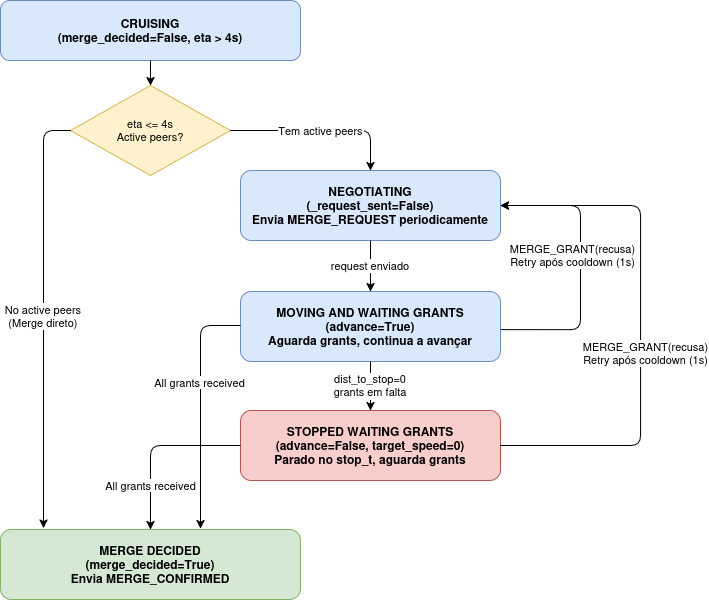
\includegraphics[width=0.85\linewidth]{mc_state_machine.png}
  \caption{Máquina de estados do Merge Car.}
  \label{fig:mc-fsm}
\end{figure}

\subsubsection{Lado do veículo da via principal}
\label{sec:lado-estrada}

Um veículo da via principal está normalmente em \textbf{IDLE} (Figura~\ref{fig:road-fsm}).
Ao receber um \textsc{merge\_request}, entra em \texttt{\_on\_merge\_request} e \textbf{avalia
o conflito}. Reconstrói a zona a partir dos \emph{waypoints} do TRR (somando os \emph{offsets}
à posição do MC) e projeta-a na sua própria estrada com \texttt{project\_t}, obtendo
$\texttt{cz\_t\_start}$ e $\texttt{cz\_t\_end}$. Calcula então os instantes em que entra e
sai da zona,
\[
  \texttt{t\_enter}=\texttt{time\_to\_cover\_distance}(v,v,d_{\text{enter}}),\quad
  \texttt{t\_exit}=\texttt{time\_to\_cover\_distance}(v,v,d_{\text{exit}}),
\]
e compara-os com a janela de ocupação do MC, $[\texttt{mc\_eta\_start},\texttt{mc\_eta\_end}]$.
O conflito é uma \textbf{sobreposição temporal}:
\[
  \texttt{in\_conflict} = (\texttt{t\_enter} < \texttt{mc\_eta\_end}) \;\wedge\;
                          (\texttt{t\_exit} > \texttt{mc\_eta\_start}).
\]

\paragraph{Sem conflito.} O veículo responde de imediato com \textsc{merge\_grant}(aceitar)
ao MC e regressa a \textbf{IDLE} --- não precisa de abrandar.

\paragraph{Com conflito.} Calcula a velocidade-alvo \texttt{\_calculate\_target\_speed}
(busca binária, Secção~\ref{sec:algoritmos}) e guarda-a em \texttt{\_pending\_speed}. Depois
procura um veículo imediatamente atrás (\texttt{find\_vehicle\_behind}):
\begin{itemize}[noitemsep,topsep=2pt]
  \item \textbf{há veículo atrás} $\rightarrow$ propaga a cadeia
        (\textbf{CHAIN\_PROPAGATING}): envia-lhe \textsc{slowdown\_request} com a sua
        sugestão e fica em \textbf{WAITING\_ACK} à espera do \textsc{slowdown\_grant};
  \item \textbf{não há veículo atrás} (fim da cadeia) $\rightarrow$ verifica a própria
        viabilidade com \texttt{can\_brake\_in\_time}: se consegue travar, compromete-se
        ($\texttt{\_slowed\_down}=\text{True}$) e envia \textsc{merge\_grant}(aceitar);
        senão, \textsc{merge\_grant}(recusar).
\end{itemize}

\paragraph{Propagação a montante.} \texttt{\_on\_slowdown\_request} replica esta lógica num
veículo intermédio: adota a velocidade sugerida (ou $0{,}7\,v$ por omissão), e ou reenvia
\textsc{slowdown\_request} ao seguinte, ou --- se for o fim da cadeia --- testa a sua
travagem e responde com \textsc{slowdown\_grant}. Quando o \textsc{slowdown\_grant}
\emph{regressa} pela cadeia, \texttt{\_on\_slowdown\_grant} confirma que a \emph{própria}
travagem continua viável e propaga-o para a frente; o veículo no topo de cada cadeia (sem
remetente à frente) traduz esse grant final no \textsc{merge\_grant} que envia ao MC. Assim,
um veículo em conflito só concede a passagem ao MC depois de garantir que toda a cadeia atrás
de si consegue abrandar em segurança.

\paragraph{Execução e retoma.} O \texttt{\_pending\_speed} é apenas \emph{pendente}: só é
efetivamente aplicado (passa a \textbf{COMMITTED}) quando chega \textsc{merge\_confirmed}(agree)
em \texttt{\_on\_merge\_confirmed} --- a partir daí, \texttt{tick()} devolve essa velocidade
ao laço de movimento e o veículo desacelera. Um \textsc{merge\_confirmed}(abort) cancela o
abrandamento e devolve-o a \textbf{IDLE}. Por fim, ao receber \textsc{execution\_status}
(\texttt{\_on\_execution\_status}, o MC já entrou na via), limpa \texttt{\_slowed\_down}/%
\texttt{\_pending\_speed} e retoma a velocidade-limite da estrada.

\begin{figure}[H]
  \centering
  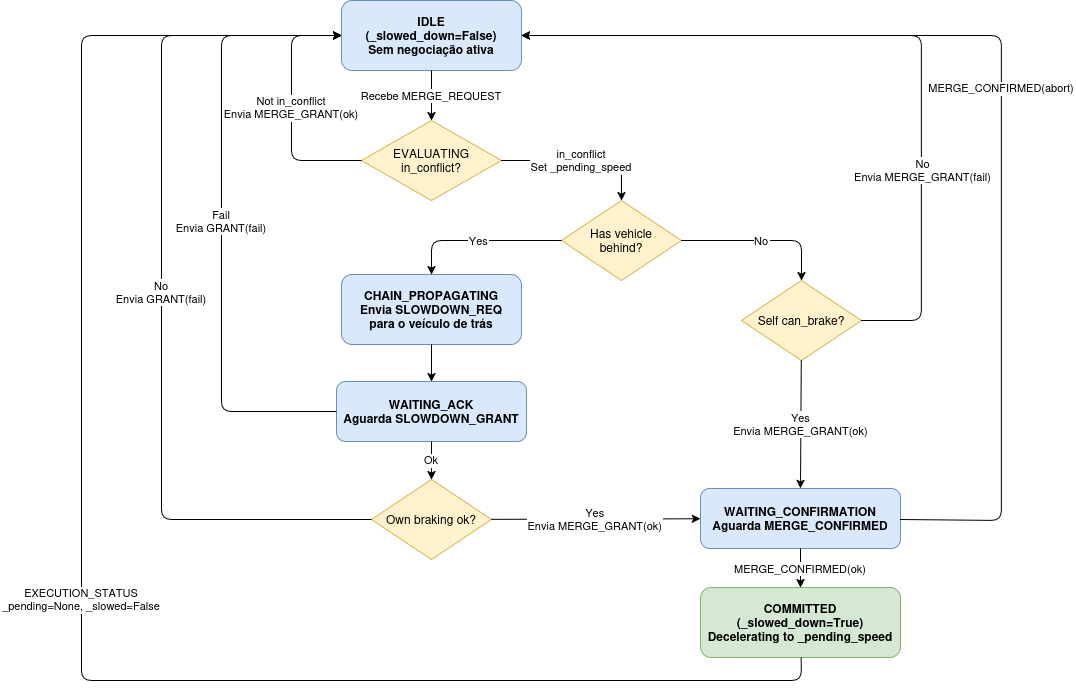
\includegraphics[width=\linewidth]{MAIN_ROAD_STATES.png}
  \caption{Máquina de estados do veículo na via principal.}
  \label{fig:road-fsm}
\end{figure}

\subsection{Algoritmos de decisão e pseudo-código}
\label{sec:algoritmos}

Três algoritmos sustentam a negociação: a deteção de conflito (O3), o cálculo da
velocidade-alvo (O4) e a propagação em cadeia do abrandamento (O4).

\paragraph{(a) Deteção de conflito.} Formaliza o teste de sobreposição temporal da
Secção~\ref{sec:lado-estrada}: o veículo só está em conflito se a janela em que ocupa a
zona intersetar a janela anunciada pelo MC.

\begin{algorithm}[H]
\caption{Deteção de conflito (\texttt{\_on\_merge\_request})}
\KwIn{posição $t$, velocidade $v$, zona $[\texttt{cz\_t\_start},\texttt{cz\_t\_end}]$,
      janela do MC $[\texttt{eta}_s,\texttt{eta}_e]$, comprimento $L_{\text{veh}}$, $L$}
\KwOut{\texttt{in\_conflict} $\in \{\text{V},\text{F}\}$}
$d_{\text{enter}} \leftarrow \max(0,\ (\texttt{cz\_t\_start}-t)\,L - L_{\text{veh}}/2)$\;
$d_{\text{exit}}  \leftarrow \max(0,\ (\texttt{cz\_t\_end}-t)\,L + L_{\text{veh}}/2)$\;
$\texttt{t\_enter} \leftarrow \texttt{time\_to\_cover\_distance}(v,v,d_{\text{enter}})$\;
$\texttt{t\_exit}  \leftarrow \texttt{time\_to\_cover\_distance}(v,v,d_{\text{exit}})$\;
\Return $(\texttt{t\_enter} < \texttt{eta}_e)\ \wedge\ (\texttt{t\_exit} > \texttt{eta}_s)$\;
\end{algorithm}

\paragraph{(b) Velocidade-alvo por busca binária.} \texttt{\_solve\_target\_speed} procura a
\emph{maior} velocidade constante-objetivo que mantém a frente do veículo ainda \emph{antes}
do início da zona no instante em que o MC a ocupa (o ETA). Usa o modelo cinemático real
(\texttt{predict\_motion}, com aceleração limitada) e $24$ iterações de bisseção --- mais do
que suficiente para convergência ao centímetro/segundo. Maximizar a velocidade minimiza o
abrandamento imposto, mantendo a fluidez (O4).

\begin{algorithm}[H]
\caption{Velocidade-alvo (\texttt{\_solve\_target\_speed})}
\KwIn{distância à zona $d$, ETA do MC \texttt{eta}, velocidade atual $v$, limite $v_{\max}$}
\KwOut{velocidade-alvo}
\lIf{$\texttt{eta} \le 0$ \textbf{ou} $d \le 0$}{\Return $0$}
$lo \leftarrow 0$;\quad $hi \leftarrow \max(v, v_{\max})$\;
\For{$24$ vezes}{
  $mid \leftarrow (lo+hi)/2$\;
  $(d_{\text{pred}},\,\_) \leftarrow \texttt{predict\_motion}(v,\,mid,\,\texttt{eta})$\;
  \lIf{$d_{\text{pred}} > d$}{$hi \leftarrow mid$}
  \lElse{$lo \leftarrow mid$}
}
\Return $hi$\;
\end{algorithm}

\paragraph{(c) Propagação em cadeia.} O abrandamento alastra de trás para a frente: cada
veículo só se compromete depois de garantir que quem está atrás de si também consegue
abrandar, e o topo da cadeia traduz esse acordo num \textsc{merge\_grant} ao MC. O
pseudo-código abaixo unifica \texttt{\_on\_merge\_request} (cabeça), \texttt{\_on\_slowdown\_request}
(propagação) e \texttt{\_on\_slowdown\_grant} (retorno).

\begin{algorithm}[H]
\caption{Propagação em cadeia do abrandamento}
\KwIn{velocidade-alvo $v_{\text{alvo}}$, remetente à frente (ou MC)}
\texttt{\_pending\_speed} $\leftarrow v_{\text{alvo}}$\;
$b \leftarrow \texttt{find\_vehicle\_behind}(\ldots)$\;
\eIf{$b \neq \varnothing$}{
  enviar \textsc{slowdown\_request}$(b, v_{\text{alvo}})$\;
  \emph{aguardar} \textsc{slowdown\_grant} de $b$ \tcp*{\texttt{\_on\_slowdown\_grant}}
}{
  $(\text{ok},\,d_{\text{trav}}) \leftarrow \texttt{can\_brake\_in\_time}(v, v_{\text{alvo}}, d_{\text{disp}})$\;
}
\uIf{cadeia atrás aceitou \textbf{e} \emph{própria} travagem ok}{
  \texttt{\_slowed\_down} $\leftarrow$ Verdadeiro\;
  responder \textsc{grant}(aceitar) ao remetente à frente \emph{ou} \textsc{merge\_grant} ao MC\;
}\Else{
  \texttt{\_pending\_speed} $\leftarrow \varnothing$\;
  responder \textsc{grant}(recusar) / \textsc{merge\_grant}(recusar)\;
}
\end{algorithm}

\subsection{Diagrama de sequência do protocolo}
\label{sec:sequencia}

A Figura~\ref{fig:seq} integra os dois lados num cenário concreto: o MC funde-se na via
onde circulam A, B e C (A à frente, C atrás), estando apenas \textbf{B em conflito}. A
sequência decorre como se segue:

\begin{enumerate}[noitemsep,topsep=2pt,label=\arabic*.]
  \item \textbf{Pedido.} Ao atingir o horizonte de $4$\,s, o MC difunde \textsc{merge\_request}
        a todos (A, B, C), com a zona de conflito e a janela de ocupação.
  \item \textbf{Grants diretos.} A e C avaliam o conflito e, não se sobrepondo à janela do
        MC, concedem \textsc{merge\_grant} de imediato.
  \item \textbf{Conflito e cadeia.} B deteta sobreposição, calcula a velocidade-alvo e,
        tendo C atrás de si, envia-lhe \textsc{slowdown\_request} em vez de responder já ao
        MC.
  \item \textbf{Retorno da cadeia.} C (fim de cadeia) confirma que trava a tempo e devolve
        \textsc{slowdown\_grant} a B; B valida a própria travagem e só então envia o seu
        \textsc{merge\_grant} ao MC.
  \item \textbf{Confirmação.} Com $\texttt{active\_peers}=\{A,B,C\}\subseteq\texttt{grants\_received}$,
        o MC difunde \textsc{merge\_confirmed}(agree). B (e a sua cadeia) aplica então o
        abrandamento; o MC executa a inserção.
  \item \textbf{Retoma.} Já na via principal, o MC emite \textsc{execution\_status} e todos
        os veículos retomam a velocidade normal.
\end{enumerate}

\paragraph{Ramo alternativo (ABORT).} Se C não conseguir travar a tempo, devolve
\textsc{slowdown\_grant}(recusar); B propaga a recusa como \textsc{merge\_grant}(recusar)
ao MC. O MC reage com \textsc{merge\_confirmed}(abort), repõe o estado e volta a tentar
após o \emph{cooldown} de $1$\,s --- ou, se entretanto alcançar o \texttt{stop\_t}, recorre
ao \emph{stop-and-wait} (Secção~\ref{sec:lado-mc}).

\begin{figure}[H]
  \centering
  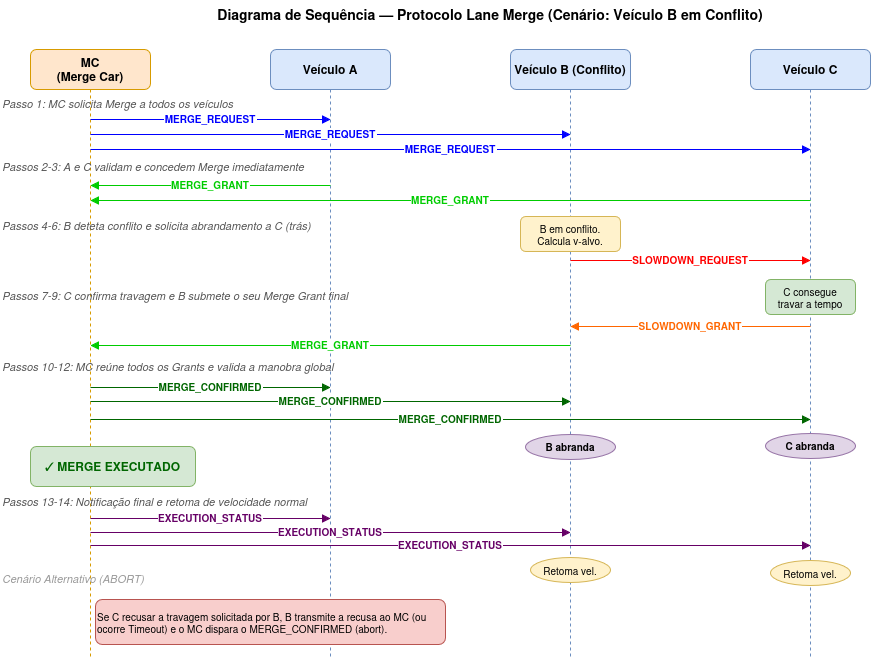
\includegraphics[width=\linewidth]{SCENARIO1_SEQ_DIAGRAM.png}
  \caption{Diagrama de sequência do protocolo (cenário com o veículo B em conflito).}
  \label{fig:seq}
\end{figure}

\subsection{Orquestração e visualização}
\label{sec:orquestracao}

Em torno da lógica de veículo existem dois componentes de suporte, que não participam na
negociação.

\paragraph{Coordenação (\texttt{coordinator.py}).} Uma GUI Tkinter lê os cenários de
\texttt{scenarios/*.json}, e ao selecionar um publica-o em \texttt{coordinator/scenario}
no router Zenoh. Cada container de veículo subscreve esse tópico e, se o seu
\texttt{station\_id} constar de \texttt{active\_vehicles}, corre o cenário, emitindo
\emph{heartbeats} em \texttt{coordinator/ready/<sid>} e, no fim, \texttt{coordinator/done/<sid>}.
O coordenador aguarda o \emph{done} de todos antes de avançar. Expõe ainda dois
interruptores: \textbf{Demo Mode} (ativa o \texttt{DemoMergeProtocol},
Secção~\ref{sec:modo-demo}) e \textbf{Draw Exag} (fator de exagero visual enviado à
\emph{dashboard}). O \texttt{run.sh} encadeia todo o arranque: \texttt{docker-compose up},
\emph{bridge}, servidor HTTP, a GUI e o browser.

\paragraph{Visualização (\texttt{bridge.py} + \texttt{dashboard.html}).} O \texttt{bridge.py}
é o único componente que fala simultaneamente Zenoh e WebSocket. Subscreve
\texttt{vanetza/out/\{cam,mcm\}} e \texttt{coordinator/scenario}, mantém o estado de cada
veículo e difunde uma trama JSON a cada $100$\,ms pela porta $8765$ para a
\texttt{dashboard.html} (\emph{canvas} HTML, sem mapas). A função \texttt{\_classify\_mcm}
traduz cada MCM num rótulo legível (e.g.\ \textsc{merge\_request}, \textsc{slowdown\_grant}),
e o estado visual de cada veículo (\textsc{normal}, \textsc{slowing}, \textsc{speeding},
\textsc{merging}) é inferido do sinal da aceleração anunciada na CAM e das transições
\textsc{merge\_confirmed}/\textsc{execution\_status}. O \emph{merge point} é recalculado
geometricamente por \texttt{\_compute\_merge\_point} (interseção das retas \texttt{main} e
\texttt{ramp}), e a zona de conflito é reconstruída a partir dos \emph{waypoints} do
\textsc{merge\_request} (O7).

\subsection{Modo Demo}
\label{sec:modo-demo}

Para tornar a negociação observável passo a passo, \texttt{protocol\_demo.py} define
\texttt{DemoMergeProtocol}, uma subclasse de \texttt{MergeProtocol}. A ideia é introduzir
pausas \emph{apenas} nos pontos de decisão relevantes: ao receber uma MCM, o
\emph{callback} determina se este veículo a vai realmente processar (\texttt{will\_process}
--- e.g.\ um \textsc{merge\_request} que lhe diz respeito, ou um \textsc{slowdown\_request}
endereçado ao seu \texttt{executantID}) e, nesse caso, dorme \texttt{demo\_pause\_s} antes
de delegar no \emph{callback} do progenitor. Os veículos da via principal congelam o
movimento (\texttt{\_demo\_paused}) ao verem o \textsc{merge\_request} e retomam-no ao
\textsc{merge\_confirmed}. Para acomodar estas pausas, o reenvio do \textsc{merge\_request}
é estrangulado a $\texttt{\_demo\_resend\_s}=1 + 4\cdot\texttt{demo\_pause\_s}$, em vez do
$1$\,s do modo normal.

% ═════════════════════════════════════════════════════════════════════════════
\section{Fluxo da Demonstração}
\label{sec:demo}

\subsection{Preparação}
\todo{run.sh; escolher cenário no coordinator; dashboard aberta.}

\subsection{Timeline}
\todo{Ponto de partida $\rightarrow$ MERGE\_REQUEST ao atingir o horizonte de 4~s
$\rightarrow$ decisões em função das mensagens recebidas $\rightarrow$ abrandamento/merge
$\rightarrow$ retoma de velocidade. Como termina a demo.}

\subsection{Aleatoriedade e variáveis}
\todo{Aleatório: manoeuvreId do SLOWDOWN\_GRANT (128--255), jitter de rede e ordem de
chegada de CAMs/MCMs. Controlável: cenário (posições iniciais), Demo Mode + pausa, Draw
Exag, speed limits e comprimentos no JSON.}

\subsection{Cenários}
\todo{Tabela dos 6 cenários: 01 standard; 02 colisão B; 03 colisão A+B+C; 04 2-MC
standard; 05 2-MC colisão B; 06 2-MC colisão todos — com o resultado esperado de cada.}

% ═════════════════════════════════════════════════════════════════════════════
\section{Resultados}
\label{sec:resultados}

\todo{Por cenário: comportamento observado (conflito, cadeia de abrandamento, merge sem
colisão) com evidência (screenshots da dashboard + logs anotados). Validação dos casos
de colisão (sem protocolo colidiria; com protocolo é seguro). Caso de abort + retry.
Caso fallback stop-and-wait. Multi-MC (cadeia também na rampa). Discussão: limitações e
simplificações do modelo.}

% ═════════════════════════════════════════════════════════════════════════════
\section{Conclusão}
\label{sec:conclusao}

\todo{Síntese do alcançado vs objetivos; lições aprendidas; trabalho futuro.}

% ═════════════════════════════════════════════════════════════════════════════
\bibliographystyle{plain}
\bibliography{referencias}

\end{document}
